%to do
\section{evaluation}
\label{sec:evaluation}

\begin{figure}
\centering
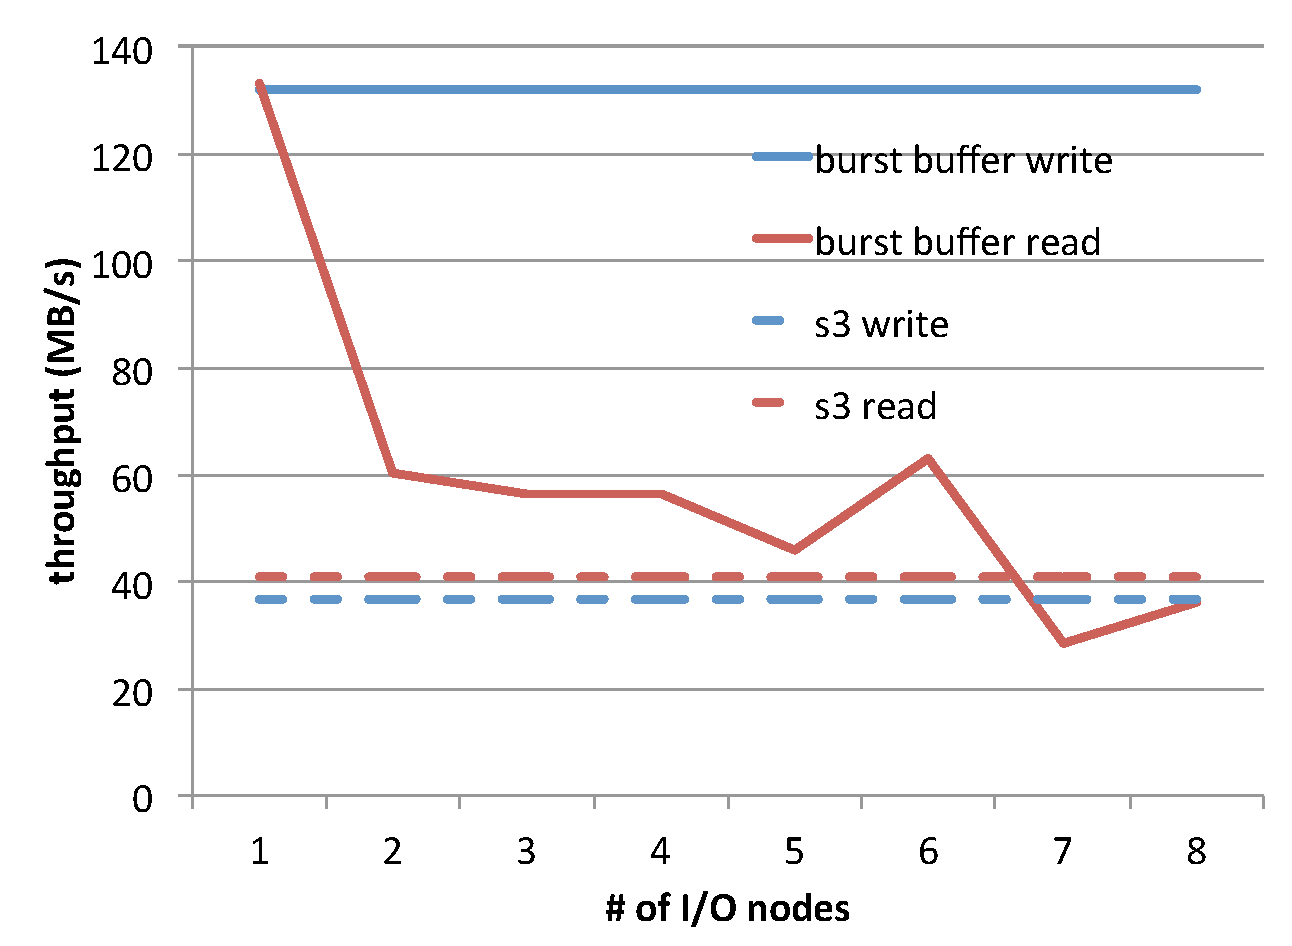
\includegraphics[width=8.5cm]{img/one_client.pdf}
\caption{One User Performance}
\label{evaluation:one user}
\end{figure}

\begin{figure}
\centering
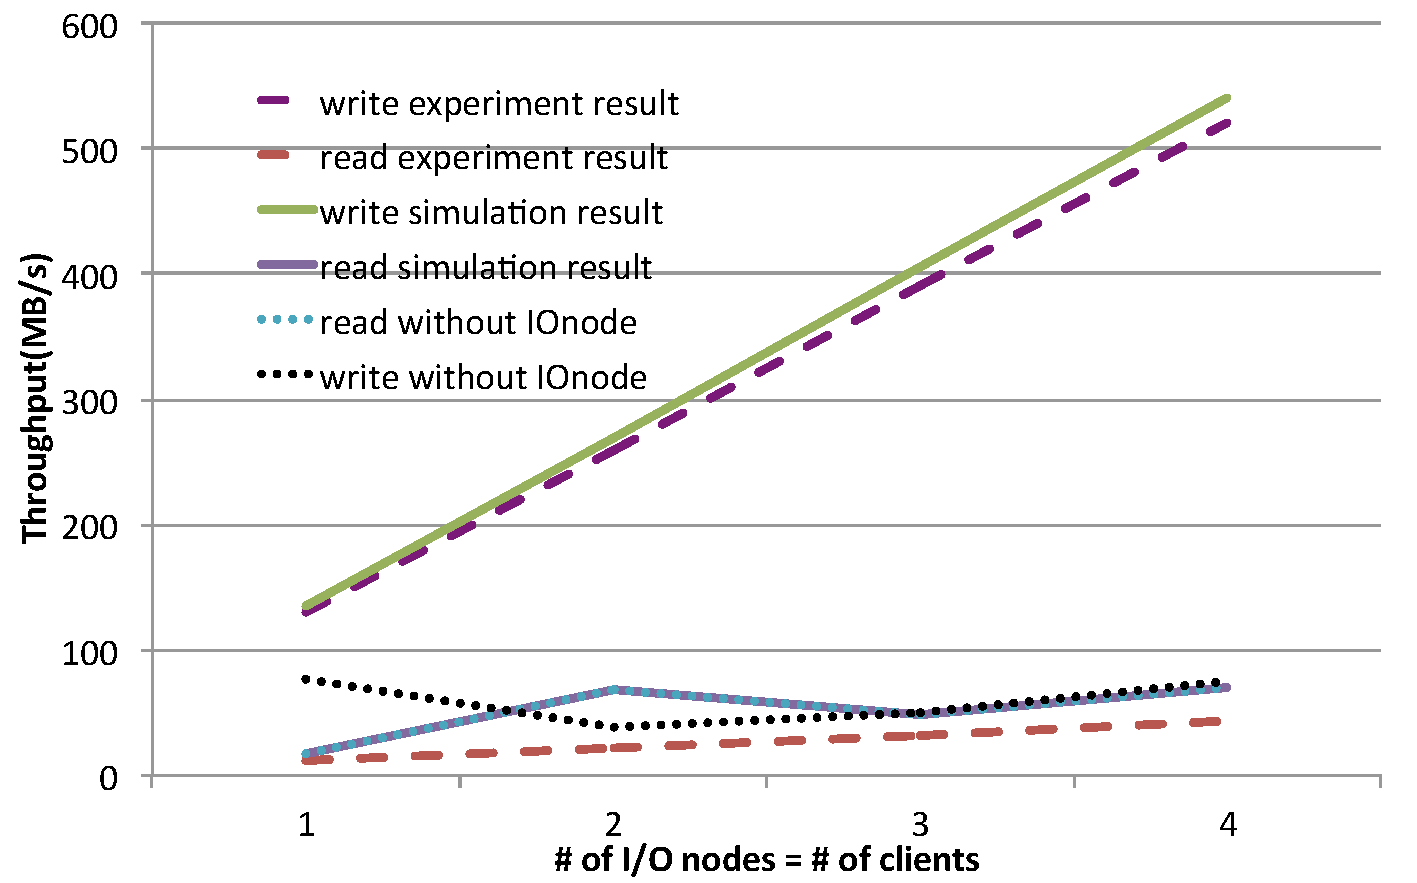
\includegraphics[width=8cm]{img/multiple_client.pdf}
\caption{Multiple User Performance}
\label{evaluation:multi user}
\end{figure}

In this section we introduce the evaluation result of our prototype implementation in Amazon EC2 public cloud.
The cloud environment is shown as Table.\ref{evaluation:environment}
\begin{table}[h]
\centering
\begin{tabular}{|c|c|}
Region				&		Tokyo		\\
Instance Type		&		m3.xlarge	\\
vCPUs				&		4			\\
ECUs				&		13			\\
Memory				&		15GiB		\\
Instance Storage	&		2*40GB(SSD)	\\
Network Performance	&		High		\\
\end{tabular}
\caption{evaluation environment}
\label{evaluation:environment}
\end{table}
here vCPUs means the number of virtual CPU in instance, and one ECU provides the equivalent CPU capacity of a 1.0-1.2GHz 2007 Opteron or 2007 Xeon processor.
For the storage system, we used a machine inside our lab

\subsection{One User Performance}
First we measure the performance of our implementation for only one user.
In this experiment, fix the number of client to one, and measure the performance for different 
number of I/O nodes. Figure~.\ref{evaluation:one user}

\subsection{Multiple Users Performance}
Our architecture can burst I/O performance for multiple users
X: number of client=number of I/O nodes Y:throughput

\subsection{Simulation for applications}
Show our architecture can burst I/O performance for applications
x